\chapter{Implementación}
\section{Prueba de concepto}
Explicar que una fase inicial del proyecto fue la prueba de concepto donde se demostró que las herramientas integradas funcionan en conjunto. Introducir brevemente el hecho de que inicialmente hubo problemas con algunas tecnologías, pero no entrar en detalles. Explicar las decisiones que se han tenido que tomar en resumidas cuentas.


\section{Prototipo real}
\textbf{Integración de Talend con JHipster: }\par
Lo primero que se hizo fue implementar un simple proceso mediante la interfaz gráfica de Talend. Este proceso realiza las siguientes operaciones: 
\begin{enumerate}
\item Descarga desde la web del \textit{Mapama} el fichero excel de los productos fitosanitarios autorizados.
\item Convierte dicho excel a un formato openoffice para poder ser procesado desde Talend con los componentes excel correspondientes. 
\item Sube a Hadoop una versión sin procesar del fichero
\item Procesa el fichero añadiendole una columna llamada ID al principio y lo sube como versión procesada a Hadoop. 
\end{enumerate} 

A continuación se exportó el proceso desde Talend: 
\textit{Archivo $\rightarrow$ Export $\rightarrow$ Java $\rightarrow$ JAR file}. Esto exporta las clases y librerias que Talend necesita para lanzar el job en un archivo comprimido llamado <nombre\_job>.jar
El siguiente paso fue descomprimir el JAR en cuestión, analizar su contenido y ver cómo se podría importar en un proyecto Java. El JAR contenía varias carpetas y ficheros pero lo que interesa es lo siguiente:
\bigskip
\par 
\dirtree{%
.1 Nombre\_del\_jar.
.2 lib.
.3 \textit{librerias jar}.
.2 Nombre\_del\_proyecto.
.3 Nombre\_del\_job.
.4 \textit{clase java principal del job}.
.2 routines.
.3 system.
.4 api.
.5 \textit{clases java}.
.4 xml.
.5 sax.
.6 \textit{clases java}.
.4 \textit{clases java}.
.3 \textit{clases java}.
}
\bigskip
\par
Así pues, a continuación se creó un nuevo proyecto Java con IntelliJ y Maven (TalendCrawler) y se copiaron todas las clases Java con su correspondiente estructura de carpetas. Dentro del fichero pom.xml del proyecto TalendCrawler donde se importaron todas las dependencias de Talend que figuraban como librerías locales en la carpeta lib. Para ello se tuvo que definir el \textit{repositorio de Cloudera} \cite{cloudera}, que es desde donde Maven buscaría la mayoría de librerías. Tras comprobar que la aplicación arrancaba y se comportaba correctamente, el próximo paso fue encapsular y exportar la aplicación como un Jar, en conjunto con sus librerías. Para ello se hizo uso del plugin \textit{one-jar} de Maven que recoge las dependencias del proyecto y las empaqueta junto a las otras clases en un único jar.\par 

En el proyecto de JHipster lo que se hizo fue crear una clase llamada Talend, desde la que periódicamente (mediante @Scheduled) se ejecutaba el Jar anterior a través del comando Runnable. 
\bigskip



\par 
\textbf{Primera versión de una integración completa}
\par
Teniendo ya el proceso de Talend integrado en la aplicación de JHipster, el siguiente problema a abordar fue el de la automatización de su ejecución. Se sabe que los productos fitosanitarios autorizados son actualizados periódicamente en la web de \textit{Mapama}. Por eso mismo, nuestra aplicación requería también de una descarga periódica de dichos datos, para asegurarse de que en todo momento el programa tiene la versión actualizada de los fitosanitarios autorizados de España. Esto se consiguió gracias al \textit{módulo de scheduling}\cite{spring_scheduling} de \textit{Spring} que permite programar la ejecución de un método de manera periódica. Como decisión estratégica se propuso lanzar el proceso de Talend cada media hora. Resuelto este problema también, el siguiente objetivo fue automatizar toda la ejecución del proceso; desde la descarga del fichero de los productos autorizados hasta la visualización de los datos mediante JHipster. Aprovechandose del mismo módulo anterior de scheduling, el desarrollo tendría que seguir el siguiente esquema: Primero, los datos deberían descargarse y procesarse mediante el módulo TalendJob. A continuación, se debería implementar otro módulo encargado de la carga de dichos datos procesados a una tabla de Hive. Después de eso, se deberían transferir los datos de Hive a la base de datos MySQL que emplea JHipster. Así pues, para cada uno de los módulos mencionados se creó un paquete con una clase que contenía los métodos necesarios para lograr sus tareas particulares. A continuación se adjunta un diagrama de clases para ilustrar de una mejor forma los módulos anteriores.


\begin{figure}[H]
    \centering
    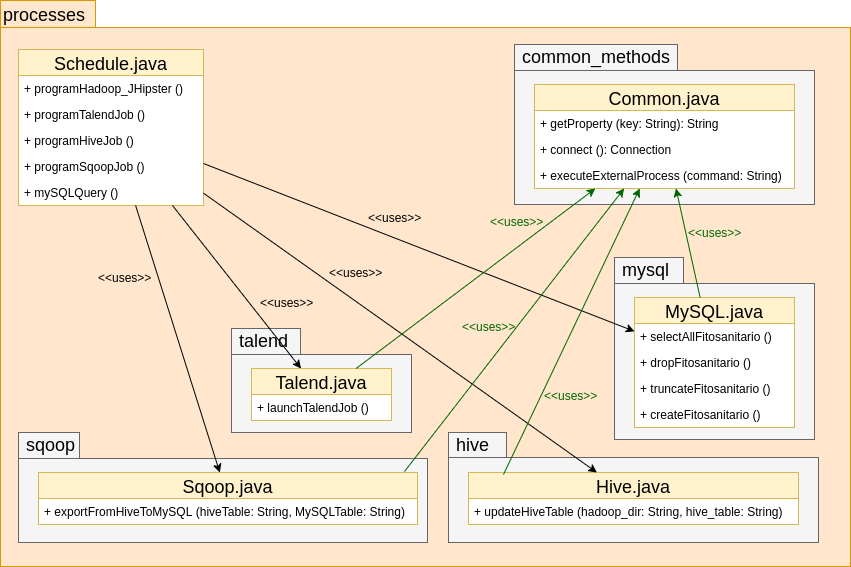
\includegraphics[width=1\textwidth]{Imagenes/Paquete_processes}
    \caption{Diagrama de clases}
    \label{fig:diag_clases}
\end{figure}
\par

\textbf{INCOMPLETO}

\bigskip
\par 
\textbf{Fichero de configuración}
\par
Para simplificar el acceso a los recursos se ha hecho uso de un fichero de configuración a los que acceden varios componentes: En primer lugar, el script bash que descarga los datos de los productos autorizados del \textit{Mapama} \cite{mapama}. Este Script usa una función bash para solicitar los valores del fichero de propiedades de la web del \textit{Mapama}, y saber la ruta en el sistema donde guardar dicho fichero. Si en cualquier momento se quiere modificar dicha localización, gracias al fichero de configuración, el único sitio que se debería modificar sería en el propio fichero. 
\par En segundo lugar, la aplicación Java del Job de Talend también accede a dicho fichero de configuración, puesto que en él se han establecido tanto rutas de almacenamiento dentro del HDFS de Hadoop, como el nombre del nodo o del usuario. No obstante, tal como se ha comentado en el apartado anterior, esta aplicación Java ha tenido que ser empaquetada en un Jar único y conjunto con todas sus librerías. Entonces ... ¿cómo accede a dicho fichero de configuración?. La solución ha sido hacer que el Jar reciba la ruta a dicho fichero mediante un argumento, de forma robusta, tal que si no recibe argumentos, o si el fichero que se le pasa no es un fichero de propiedades, el proceso alerta del error y se detiene. 
\bigskip
\par
\textit{Explicar en detalle el funcionamiento típico de la aplicación y la presentación de los datos. Hacer una especie de manual del usuario resumido y si hay algún aspecto interesante de la aplicación, hacer hincapié en el.}
\section{Problemas técnicos detectados}
Mencionar los problemas confrontados durante la realización del proyecto y la manera en la que se han solucionado.
